\documentclass[11pt]{article}

%	packages
\usepackage{amsmath}
\usepackage{amssymb} 
\usepackage{caption}
\usepackage{graphicx}
\usepackage{subcaption}
\usepackage{tikz}
\usetikzlibrary{arrows}
\usetikzlibrary{decorations.markings}
\usepackage{pgfplots}
\usetikzlibrary{pgfplots.groupplots}
\pgfplotsset{compat=1.3}
\usetikzlibrary{calc}
\usetikzlibrary{matrix}
\newcommand{\midarrow}{\tikz \draw[ultra thick, -triangle 45] (0,0) -- +(.1,0);}
\newcommand{\midarrowThick}{\tikz \draw[-stealth', thick] (0,0) -- +(.1,0);}



%%%%%%%%%%%%%%%%%%%%%%%%%%%%%%%%%%%%%%%%%%%%%%%%%%%%%%%%%%%%%%%%%%%%%%%%%%%
% Tables for data
%%%%%%%%%%%%%%%%%%%%%%%%%%%%%%%%%%%%%%%%%%%%%%%%%%%%%%%%%%%%%%%%%%%%%%%%%%%

% # bi stability
%# D,h = 1.0,0.5

\pgfplotstableread{
Disease Harshness
1.0 0.49
0.98 0.5
0.75 0.6
0.58 0.68
0.39 0.78
0.22 0.88
0 1.0
}{\altruismUnstable}

\pgfplotstableread{
Disease Harshness
1 0.7
0.95 0.72
0.9 0.73
0.85 0.75
0.8 0.77
0.78 0.78
%0.75 0.78
0.72 0.8
%0.47 0.9
%0.23 1.0
0.4 0.88
0.3 0.91
0.2 0.95
0 1.0
% these are limit points->where the saddle meets the node
%0.78 0.78 % limit point
%0.72 0.8  % limit point
%0.47 0.9 % limit point
%0.23 1.0 % limit point
}{\altruismStable}


\pgfplotstableread{
Disease Harshness
0 1
0.2 0.95
0.3 0.91
0.4 0.88
0.5 0.84
0.6 0.82
0.7 0.79
0.8 0.77
0.78 0.78
%0.75 0.78
0.72 0.8
0.47 0.9
0.23 1.0
0 1.0
% the birth of unstable state
% i.e. where both stable and unstable exits
% the birth of unstable state
% i.e. where both stable and unstable exits
}{\altruismSN}

\pgfplotstableread{
Disease Harshness
0 1
0.2 0.95
0.3 0.91
0.4 0.88
0.5 0.84
0.6 0.82
0.7 0.79
0.8 0.77
0.9 0.73
0.95 0.72
1 0.7
}{\emptyStable}

\pgfplotstableread{
Disease Harshness
0 0.99
0.2 0.91
0.3 0.88
0.4 0.85
0.5 0.81
0.6 0.78
0.7 0.74
0.8 0.71
0.9 0.68
1.0 0.64
}{\selfishUnstable}

\pgfplotstableread{
Disease Harshness
0 1
0.1 0.96
%0.2
0.3 0.86
0.38  0.8
0.57 0.7
0.8  0.6
1 0.5
% ustable branch appears when cont H alturist limit point enters the fesible domain, i.e. when it is less than 1 
}{\selfishStable}

% selfish stable alt unstable empty unstable
\pgfplotstableread{
Disease Harshness
0 1
1 0.48 
}{\I}

% selfish stable alt stable empty unstable
\pgfplotstableread{
Disease Harshness
0 1
0.1 0.965
1 0.5
}{\II}

% selfish unstable alt stable empty unstable
\pgfplotstableread{
Disease Harshness
0.0 1
1 0.64
}{\III}

% alt SN empty stable
\pgfplotstableread{
Disease Harshness
0 1
0.3 1
1 0.7
}{\IVa}

% alt SN LP beyond feasible region empty stable
\pgfplotstableread{
Disease Harshness
0 1
0.3 1
0.3 0.89
}{\IVb}

% empty stable
\pgfplotstableread{
Disease Harshness
0.3 1
1 0.7
}{\V}



\pagestyle{empty}
\begin{document}

%\pgfplotsset{
%% override style for non-boxed plots
%    % which is the case for both sub-plots
%    every non boxed x axis/.style={} 
%}



\begin{figure}
\hspace*{-10em}
	\centering
	\begin{tikzpicture}[scale=2]
	\matrix{
		\begin{axis}[
			xlabel=Disease,
			ylabel=Harshness,
			title={Altruists},
			%width=0.45\textwidth,
			xmin=0, xmax=1,
			ymin=0, ymax=1,
			mark size=1.25pt
			%legend cell align=left,
			%legend pos=outer north east, 
			%legend style={draw=none}
		]		
		
		% stable sharded area
		
		
		\addplot[fill=white] 
			plot [] coordinates {(0,1) (1,1) }
			\closedcycle;	
		\addplot[] 
			plot [x=Disease, y = Harshness] table [] {\V} ;	
		\addplot[fill=red!50] 
			plot [x=Disease, y = Harshness] table [] {\IVa} \closedcycle;
		\addplot[] 
			plot [x=Disease, y = Harshness] table [] {\IVb};
		\addplot[fill=red!30] 
			plot [x=Disease, y = Harshness] table [] {\III}\closedcycle;
		%\addplot[fill=black!30] 
		%	plot [x=Disease, y = Harshness] table [] {\II} \closedcycle;
		\addplot[fill=blue!30] 
			plot [x=Disease, y = Harshness] table [] {\I}\closedcycle;
			
		
		\node[] at (axis cs:0.8,0.2) {Unstable};
		\node[] at (axis cs:0.8,0.66) {Stable};
		\node[] at (axis cs:0.8,0.9) {No Solution};
		\node[] at (axis cs:0.3,0.5) {Saddle Node};
		\draw[->, thick] (axis cs:0.3,0.55) -- (axis cs:0.4,0.9){};
		\draw[->, thick] (axis cs:0.3,0.55) -- (axis cs:0.2,0.975){};
		
		%\legend{Canonical, Repeat};
		\end{axis}
		
		&\begin{axis}[
			xlabel=Disease,
			ylabel=Harshness,
			title={Selfish},
			%width=0.45\textwidth,
			xmin=0, xmax=1,
			ymin=0, ymax=1,
			mark size=1.25pt
			%legend cell align=left,
			%legend pos=outer north east, 
			%legend style={draw=none}
		]		
		
		
		% unstable shaded area
		\addplot[fill=white] 
			plot [] coordinates {(0,1) (1,1) }
			\closedcycle;	
		\addplot[fill=blue!30] 
			plot [x=Disease, y = Harshness] table [] {\III}
			\closedcycle;
		\addplot[fill=red!30] 
			plot [x=Disease, y = Harshness] table [] {\II}
			\closedcycle;
		% unstable boundary
		% lables
		\node[] at (axis cs:0.8,0.2) {Stable};
		\node[] at (axis cs:0.8,0.67) {Unstable};
		\node[] at (axis cs:0.8,0.9) {No Solution};

		\end{axis}\\
		
		\begin{axis}[
			xlabel=Disease,
			ylabel=Harshness,
			title={Empty},
			%width=0.45\textwidth,
			xmin=0, xmax=1,
			ymin=0, ymax=1,
			mark size=1.25pt
			%legend cell align=left,
			%legend pos=outer north east, 
			%legend style={draw=none}
		]
		
		
		
		% saddle node region 
		% dead state
		\addplot[fill=red!30] 
			plot [] coordinates {(0,1) (1,1) }
			\closedcycle;	
		\addplot[fill=blue!30] 
			plot [x=Disease, y = Harshness] table [] {\III} 
			\closedcycle;	
		
		\node[] at (axis cs:0.8,0.2) {Unstable};
		\node[] at (axis cs:0.8,0.9) {Stable};	
			
		
		\end{axis}
		
		&\begin{axis}[
			xlabel=Disease,
			ylabel=Harshness,
			title={System},
			%width=0.45\textwidth,
			xmin=0, xmax=1,
			ymin=0, ymax=1,
			mark size=1.25pt
			%legend cell align=left,
			%legend pos=outer north east, 
			%legend style={draw=none}
		]
		
		\addplot[fill=green!30] 
			plot [] coordinates {(0,1) (1,1) }\closedcycle;	
		\addplot[] 
			plot [x=Disease, y = Harshness] table [] {\V} ;	
		\addplot[fill=purple!80] 
			plot [x=Disease, y = Harshness] table [] {\IVa} \closedcycle;
		\addplot[] 
			plot [x=Disease, y = Harshness] table [] {\IVb};
		\addplot[fill=green!30] 
			plot [x=Disease, y = Harshness] table [] {\III}\closedcycle;
		\addplot[fill=black!30] 
			plot [x=Disease, y = Harshness] table [] {\II} \closedcycle;
		\addplot[fill=green!30] 
			plot [x=Disease, y = Harshness] table [] {\I}\closedcycle;
			
		
		% lables
		\node[] at (axis cs:0.2,0.2) {I};
		\node[] at (axis cs:0.5,0.5) {II};
		\draw[->, ultra thick] (axis cs:0.55,0.55) -- (axis cs:0.6,0.7){};
		\node[] at (axis cs:0.9,0.62) {III};
		\node[] at (axis cs:0.4,0.91) {IVa};
		\node[] at (axis cs:0.24,0.96) {IVb};
		\node[] at (axis cs:0.9,0.9) {V};
		\end{axis}\\
	};
	\end{tikzpicture}
\end{figure}

%%%%%%%%%%%%%
% only individual agents
%%%%%%%%%%%%%

\begin{figure}
\hspace*{-10em}
	\centering
	\begin{tikzpicture}%[scale=2]
	\matrix{
		\begin{axis}[
			xlabel=Disease,
			ylabel=Harshness,
			title={Altruists},
			width=0.55\textwidth,
			xmin=0, xmax=1,
			ymin=0, ymax=1,
			mark size=1.25pt
			%legend cell align=left,
			%legend pos=outer north east, 
			%legend style={draw=none}
		]		
		
		% stable sharded area
		
		
		\addplot[fill=white] 
			plot [] coordinates {(0,1) (1,1) }
			\closedcycle;	
		\addplot[] 
			plot [x=Disease, y = Harshness] table [] {\V} ;	
		\addplot[fill=red!50] 
			plot [x=Disease, y = Harshness] table [] {\IVa} \closedcycle;
		\addplot[] 
			plot [x=Disease, y = Harshness] table [] {\IVb};
		\addplot[fill=red!30] 
			plot [x=Disease, y = Harshness] table [] {\III}\closedcycle;
		%\addplot[fill=black!30] 
		%	plot [x=Disease, y = Harshness] table [] {\II} \closedcycle;
		\addplot[fill=blue!30] 
			plot [x=Disease, y = Harshness] table [] {\I}\closedcycle;
			
		
		\node[] at (axis cs:0.8,0.2) {Unstable};
		\node[] at (axis cs:0.8,0.66) {Stable};
		\node[] at (axis cs:0.8,0.9) {No Solution};
		\node[] at (axis cs:0.3,0.5) {Saddle Node};
		\draw[->, thick] (axis cs:0.3,0.55) -- (axis cs:0.4,0.9){};
		\draw[->, thick] (axis cs:0.3,0.55) -- (axis cs:0.2,0.975){};
		
		%\legend{Canonical, Repeat};
		\end{axis}
		
		&\begin{axis}[
			xlabel=Disease,
			%ylabel=Harshness,
			title={Selfish},
			width=0.55\textwidth,
			xmin=0, xmax=1,
			ymin=0, ymax=1,
			ytick = \empty,
			mark size=1.25pt
			%legend cell align=left,
			%legend pos=outer north east, 
			%legend style={draw=none}
		]		
		
		
		% unstable shaded area
		\addplot[fill=white] 
			plot [] coordinates {(0,1) (1,1) }
			\closedcycle;	
		\addplot[fill=blue!30] 
			plot [x=Disease, y = Harshness] table [] {\III}
			\closedcycle;
		\addplot[fill=red!30] 
			plot [x=Disease, y = Harshness] table [] {\II}
			\closedcycle;
		% unstable boundary
		% lables
		\node[] at (axis cs:0.8,0.2) {Stable};
		\node[] at (axis cs:0.8,0.67) {Unstable};
		\node[] at (axis cs:0.8,0.9) {No Solution};

		\end{axis}
		
		&\begin{axis}[
			xlabel=Disease,
			%ylabel=Harshness,
			title={Empty},
			width=0.55\textwidth,
			xmin=0, xmax=1,
			ymin=0, ymax=1,
			ytick = \empty,
			mark size=1.25pt
			%legend cell align=left,
			%legend pos=outer north east, 
			%legend style={draw=none}
		]
		
		
		
		% saddle node region 
		% dead state
		\addplot[fill=red!30] 
			plot [] coordinates {(0,1) (1,1) }
			\closedcycle;	
		\addplot[fill=blue!30] 
			plot [x=Disease, y = Harshness] table [] {\III} 
			\closedcycle;	
		
		\node[] at (axis cs:0.8,0.2) {Unstable};
		\node[] at (axis cs:0.8,0.9) {Stable};	
			
		
		\end{axis}\\
	};
	\end{tikzpicture}
\end{figure}

~\\
\newpage
~\\

%%%%%%%%%%%
% system plot with Phase space plots
%%%%%%%%%%%

	\begin{figure}
	\hspace*{-15em}
	\begin{subfigure}[b]{\textwidth}

	\centering
	\begin{tikzpicture}[scale=1.1 ]
	
		\begin{axis}[
			xlabel=Disease,
			ylabel=Harshness,
			title={},
			%width=0.55\textwidth,
			xmin=0, xmax=1,
			ymin=0, ymax=1,
			mark size=1.25pt
			%legend cell align=left,
			%legend pos=outer north east, 
			%legend style={draw=none}
		]
		
		\addplot[fill=green!30] 
			plot [] coordinates {(0,1) (1,1) }\closedcycle;	
		\addplot[] 
			plot [x=Disease, y = Harshness] table [] {\V} ;	
		\addplot[fill=purple!80] 
			plot [x=Disease, y = Harshness] table [] {\IVa} \closedcycle;
		\addplot[] 
			plot [x=Disease, y = Harshness] table [] {\IVb};
		\addplot[fill=green!30] 
			plot [x=Disease, y = Harshness] table [] {\III}\closedcycle;
		\addplot[fill=black!30] 
			plot [x=Disease, y = Harshness] table [] {\II} \closedcycle;
		\addplot[fill=green!30] 
			plot [x=Disease, y = Harshness] table [] {\I}\closedcycle;
			
		
		% lables
		\node[] at (axis cs:0.2,0.2) {I};
		\node[] at (axis cs:0.5,0.5) {II};
		\draw[->, ultra thick] (axis cs:0.55,0.55) -- (axis cs:0.6,0.7){};
		\node[] at (axis cs:0.9,0.62) {III};
		\node[] at (axis cs:0.4,0.91) {IVa};
		\node[] at (axis cs:0.24,0.96) {IVb};
		\node[] at (axis cs:0.9,0.9) {V};

	
		\end{axis}
		
		\end{tikzpicture}
	\end{subfigure}%\hspace*{0.5cm}
	%%%%%%%%%%%%%%%%%%
	% Region I
	%%%%%%%%%%%%%%%%%%
	\begin{subfigure}[b]{0.3\textwidth}
	\hspace*{-2em}
	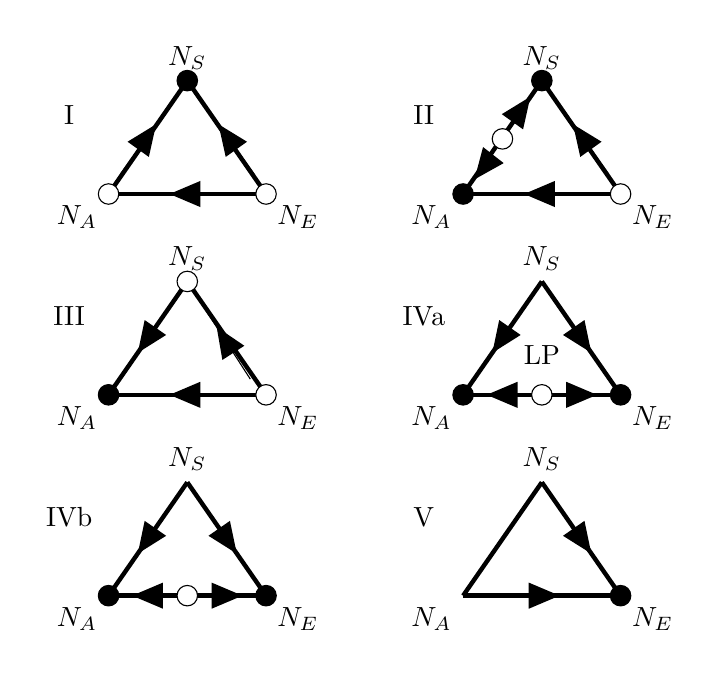
\begin{tikzpicture}[every node/.style={sloped,allow upside down} ]
		\matrix{
		
		\draw[-,ultra thick] (2,0) -- (0,0) node[below left] {$N_A$};
		\draw[-,ultra thick] (1,1.44) -- (2,0) node[below right] {$N_E$};
		\draw[-,ultra thick] (0,0) -- (1,1.44) node[above] {$N_S$};
		\node[] at (-0.5,1) {I};
		\node[] at (3.5,0) {};
		
		% trajectories
		\draw[] (0.15,0.25)-- node {\midarrow} (1,1.44);
		\draw[] (1.85,0.25)-- node {\midarrow} (1,1.44);
		\draw[] (1.65,0)-- node {\midarrow} (0,0);
		%\draw[] (0.1,0.9) to[out=270, in=90] node {\midarrowThick}
		
		% fixed point
		\draw[color=black,fill=white] (0,0) ellipse [x radius=0.13cm, y radius=0.13cm] {};
		\draw[color=black,fill=white] (2,0) ellipse [x radius=0.13cm, y radius=0.13cm] {};
		\draw[color=black,fill=black] (1,1.44) ellipse [x radius=0.13cm, y radius=0.13cm] {};
		
		&
		\draw[-,ultra thick] (2,0) -- (0,0) node[below left] {$N_A$};
		\draw[-,ultra thick] (1,1.44) -- (2,0) node[below right] {$N_E$};
		\draw[-,ultra thick] (0,0) -- (1,1.44) node[above] {$N_S$};
		\node[] at (-0.5,1) {II};
		
		% trajectories
		\draw[] (1.85,0.25)-- node {\midarrow} (1,1.44);
		\draw[] (1.65,0)-- node {\midarrow} (0,0);
		\draw[] (0.35,0.45)-- node {\midarrow} (0,0);
		\draw[] (0.65,0.95)-- node {\midarrow} (1,1.44);
		%\draw[] (0.1,0.9) to[out=270, in=90] node {\midarrowThick}
		
		% fixed point
		\draw[color=black,fill=black] (0,0) ellipse [x radius=0.13cm, y radius=0.13cm] {};
		\draw[color=black,fill=white] (2,0) ellipse [x radius=0.13cm, y radius=0.13cm] {};
		\draw[color=black,fill=black] (1,1.44) ellipse [x radius=0.13cm, y radius=0.13cm] {};
		\draw[color=black,fill=white] (0.5,0.7) ellipse [x radius=0.13cm, y radius=0.13cm] {};
		
		\\
		\draw[-,ultra thick] (2,0) -- (0,0) node[below left] {$N_A$};
		\draw[-,ultra thick] (1,1.44) -- (2,0) node[below right] {$N_E$};
		\draw[-,ultra thick] (0,0) -- (1,1.44) node[above] {$N_S$};
		\node[] at (-0.5,1) {III};
		\node[] at (3.5,0) {};
		
		% trajectories
		\draw[] (0.8,1.15)-- node {\midarrow} (0,0);
		\draw[] (1.8,0.2)-- node {\midarrow} (1,1.44);
		\draw[] (1.65,0)-- node {\midarrow} (0,0);
		%\draw[] (0.1,0.9) to[out=270, in=90] node {\midarrowThick}
		
		% fixed point
		\draw[color=black,fill=black] (0,0) ellipse [x radius=0.13cm, y radius=0.13cm] {};
		\draw[color=black,fill=white] (2,0) ellipse [x radius=0.13cm, y radius=0.13cm] {};
		\draw[color=black,fill=white] (1,1.44) ellipse [x radius=0.13cm, y radius=0.13cm] {};
		&
		\draw[-,ultra thick] (2,0) -- (0,0) node[below left] {$N_A$};
		\draw[-,ultra thick] (1,1.44) -- (2,0) node[below right] {$N_E$};
		\draw[-,ultra thick] (0,0) -- (1,1.44) node[above] {$N_S$};
		\node[] at (-0.5,1) {IVa};
		\node[] at (1,0.5) {LP};
		
		% trajectories
		\draw[] (0.7,0)-- node {\midarrow} (0,0);
		\draw[] (1.3,0)-- node {\midarrow} (2,0);
		\draw[] (0.8,1.15)-- node {\midarrow} (0,0);
		\draw[] (1.2,1.15)-- node {\midarrow} (2,0);
		
		% fixed point
		\draw[color=black,fill=black] (0,0) ellipse [x radius=0.13cm, y radius=0.13cm] {};
		\draw[color=black,fill=black] (2,0) ellipse [x radius=0.13cm, y radius=0.13cm] {};
		\draw[color=black,fill=white] (1,0) ellipse [x radius=0.13cm, y radius=0.13cm] {};
		
		\\
		\draw[-,ultra thick] (2,0) -- (0,0) node[below left] {$N_A$};
		\draw[-,ultra thick] (1,1.44) -- (2,0) node[below right] {$N_E$};
		\draw[-,ultra thick] (0,0) -- (1,1.44) node[above] {$N_S$};
		\node[] at (-0.5,1) {IVb};
		
		% trajectories
		\draw[] (0.7,0)-- node {\midarrow} (0,0);
		\draw[] (1.3,0)-- node {\midarrow} (2,0);
		\draw[] (0.8,1.15)-- node {\midarrow} (0,0);
		\draw[] (1.2,1.15)-- node {\midarrow} (2,0);
		
		% fixed point
		\draw[color=black,fill=black] (0,0) ellipse [x radius=0.13cm, y radius=0.13cm] {};
		\draw[color=black,fill=black] (2,0) ellipse [x radius=0.13cm, y radius=0.13cm] {};
		\draw[color=black,fill=white] (1,0) ellipse [x radius=0.13cm, y radius=0.13cm] {};
		
		&
		\draw[-,ultra thick] (2,0) -- (0,0) node[below left] {$N_A$};
		\draw[-,ultra thick] (1,1.44) -- (2,0) node[below right] {$N_E$};
		\draw[-,ultra thick] (0,0) -- (1,1.44) node[above] {$N_S$};
		\node[] at (-0.5,1) {V};
		
		% trajectories
		\draw[] (1.2,1.15)-- node {\midarrow} (2,0);
		\draw[] (0.35,0)-- node {\midarrow} (2,0);
		%\draw[] (0.1,0.9) to[out=270, in=90] node {\midarrowThick}
		
		% fixed point
		\draw[color=black,fill=black] (2,0) ellipse [x radius=0.13cm, y radius=0.13cm] {};
		
		\\
		};

		\end{tikzpicture}
	\end{subfigure}
	
	\end{figure}\hspace*{0.5cm}




\end{document}